\documentclass[a4paper, 12pt]{article}%тип документа

%отступы
\usepackage[left=2cm,right=2cm,top=2cm,bottom=3cm,bindingoffset=0cm]{geometry}
\setlength{\parindent}{5ex}

%Русский язык
\usepackage[T2A]{fontenc} %кодировка
\usepackage[utf8]{inputenc} %кодировка исходного кода
\usepackage[english,russian]{babel} %локализация и переносы

%Вставка картинок
\usepackage{graphicx}
\graphicspath{{pictures/}}
\DeclareGraphicsExtensions{.pdf,.png,.jpg}

%Графики
\usepackage{pgfplots}
\pgfplotsset{compat=1.9}

%Математика
\usepackage{amsmath, amsfonts, amssymb, amsthm, mathtools}

%Таблицы
\usepackage{longtable} 
\usepackage{float}

%Римские цифры
\newcommand{\RomanNumeralCaps}[1]{\uppercase\expandafter{\romannumeral#1}}

\usepackage{multirow}

\usepackage{hhline}

\begin{document}
	\begin{titlepage}
		\begin{center}
			\textsc{Федеральное государственное автономное образовательное учреждение высшего образования«Московский физико-технический институт (национальный исследовательский университет)»\\[5mm]
			}
			
			\vfill
			
			\textbf{Вопрос по выбору: \\[3mm]
				Интерферометр Жамена.
				\\[50mm]
			}
			
		\end{center}
		
		\hfill
		\begin{minipage}{.5\textwidth}
			Выполнили студенты:\\[2mm]
			Сериков Василий Романович\\[2mm]
			Группа: Б03-102\\[5mm]
			Сериков Алексей Романович\\[2mm]
			Группа: Б03-103\\[5mm]
			
		\end{minipage}
		\vfill
		\begin{center}
			Москва, 2023 г.
		\end{center}
		
	\end{titlepage}
	
	\newpage
	\textbf{Аннотация}\\
	
	
	\textbf{Цель работы: }\\
	
	Измерение показателей преломления газов с помощью интерферометра Жамена.\\
	
	\textbf{В работе используется: }\\
	
	Интерферометр Жамена, газовая кювета,
	осветитель, зрительная труба, сильфон, баллон с углекислым газом,
	манометр, краны.\\
	
	\textbf{Теория: }\\
	
	Главной частью интерферометра Жамена являются две одинаковые толстые плоскопараллельные стеклянные
	пластинки $P_1$ и $P_2$, посеребрённые с одной стороны. расположены они так, чтобы между их плоскостями был небольшой угол.
	
	\begin{figure}[H]
		\center{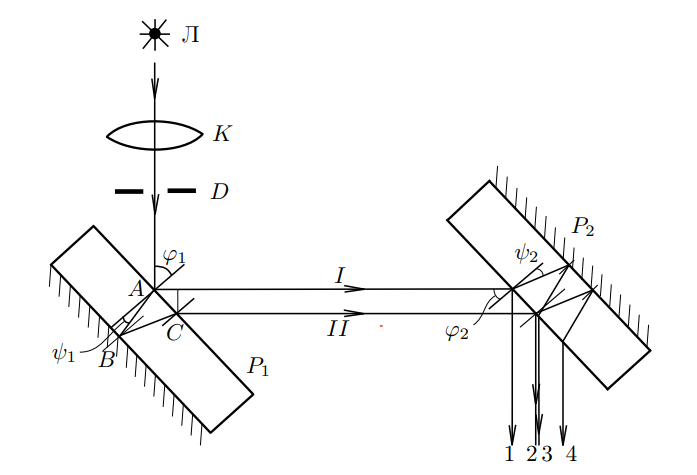
\includegraphics[scale=0.6]{ust.png}}
		\caption{Ход лучей в интерферометре Жамена}
	\end{figure}
	
	На выходе интерферометра оказывается 4 луча. Наименьшая разность хода только между лучами 2 и 3. Между остальными, в силу большой толщины пластинок, большая разность хода. Поэтому интерференция возникает только при суперпозиции лучей 2 и 3. Присутствие лучей 1 и 4 ухудшает чёткость интерференционной картины, и поэтому их устраняют с помощью диафрагм.
	
	Подсчитаем разность хода между лучами 2 и 3. Разность хода между лучами I и II, отражёнными от передней и задней поверхности пластинки $P_1$, равна
	\begin{equation}
	\Delta_1 = n(AB + BC) - AH = 2hn \cos \psi_1.
	\end{equation}
	где n — показатель преломления, h — толщина пластинки, $\psi_1$ - угол преломления в пластинке $P_1$. После отражения от поверхностей пластинки
	$P_2$ лучи 2 и 3 приобретают дополнительную разность хода, равную
	\begin{equation}
	\Delta_2 = 2hn\cos \psi_2.
	\end{equation} 
	где $\psi_2$ — угол преломления в пластинке $P_2$. Полная разность хода между
	лучами 2 и 3 равна
	\begin{equation}
	\Delta = \Delta_1 - \Delta_2 = 2hn(\cos \psi_1 - \cos \psi_2).
	\end{equation}
	
	Максимумы освещённости располагаются в тех точках
	фокальной плоскости зрительной трубы, где сходятся лучи с разностью
	хода
	$\Delta$ = m$\lambda$ (m = 0, $\pm$ 1, $\pm$ 2, . . . ). (4)
	Разность хода
	$\Delta$ = (m + 1/2)$\lambda$ (5)
	соответствует минимальной освещённости.
	При заданной геометрии прибора разность хода зависит от углов $\psi_1$
	и $\psi_2$, которые определяются углом падения световых лучей на пластинку $p_1$. При освещении расходящимся пучком света можно наблюдать систему интерференционных полос.
	
	Интерферометр Жамена можно использовать для измерения небольших изменений показателя преломления. Для этого исследуемое вещество ставят на пути одного из лучей (I или II), что вносит дополнительную разность хода и приводит к сдвигу интерференционных полос. Измерения чаще всего проводят компенсационным методом. При этом на
	пути второго луча ставят тщательно прокалиброванный компенсатор,
	положение которого подбирается так, чтобы вернуть интерференционную картину в исходное положение.\\
	
	
	\textbf{Ход работы: }\\
	
	\begin{enumerate}
		\item Проведём калибровку прибора. Для калибровки наденем на окуляр красный светофильтр и снимем зависимость показаний микрометрической шкалы компенсатора Жамена от порядкового номера интерференционного максимума. Повторим настройку нуля несколько раз, вращая винт в одну сторону, чтобы исключить люфт. Результаты усредненных измерений занесём в таблицу 1. По полученным данным построим калибровочный график\\
		
		\begin{longtable}{|c|c|c|c|c|c|c|c|c|c|c|c|}
			\hline
			m & 0 & 1 & 2 & 3 & 4 & 5 & 6 & 7 & 8 & 9 & 10 \\ \hline
			$z_m$, мм & 16,69 & 16,75 & 16,80 & 16,86 & 16,90 & 16,96 & 17,00 & 17,06 & 17,11 & 17,16 & 17,21 \\

		\hline
		\hline
		
		m & 0 & -1 & -2 & -3 & -4 & -5 & -6 & -7 & -8 & -9 & -10 \\ \hline
		$z_m$, мм & 16,69 & 16,65 & 16,60 & 16,55 & 16,50 & 16,44 & 16,40 & 16,35 & 16,30 & 16,25 & 16,20 \\ \hline
		\caption{Полученные значения для калибровки компенсатора. $\sigma_{z_m} = 0,02$ мм}
	\end{longtable}

		\begin{figure}[H]
			\center{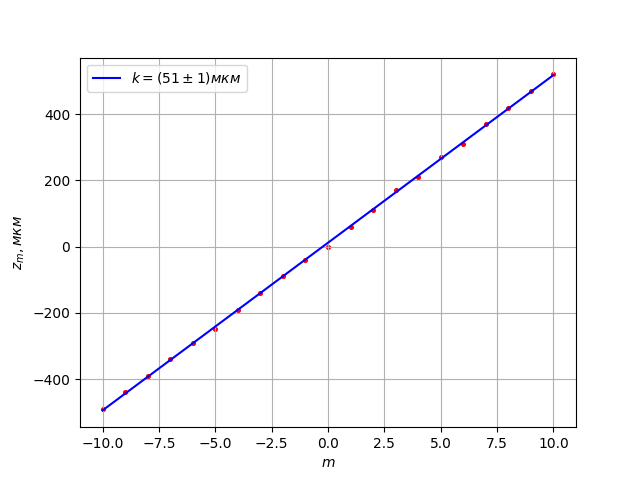
\includegraphics[scale=0.85]{z(m).png}}
			\caption{Калибровочный график для компенсатора.}
		\end{figure}
		
		
		\item Изменяя давление с помощью сильфона, снимем зависимость показаний компенсатора $z$ от перепада давлений $\triangle P$. Результаты занесём в таблицу 2.
		
		\begin{longtable}{|c|c|c|c|c|c|c|c|c|c|}
			\hline
			$P, $ кПа & -9 & -8 & -7,5 & -6,5 & -6 & -5& -4,5 & -4 & -3\\
			\hline
			$z,$ нм& 16,83 & 16,79 & 16,78 & 16,75 & 16,73 & 16,72 & 16,71 & 16,68 & 16,67  \\
			
			\hline
			\hline
			
			$P, $ кПа  -2 & -1,7 & -1 & -0,5 & 0,5 & 1,2 & 2 & 2,7 & 3,5 & 4,7  \\
			\hline
			$z,$ нм&  16,66 & 16,64 & 16,63 & 16,61 & 16,58 & 16,55 & 16,53 & 16,51 & 16,49  \\ \hline
			
			\caption{зависимость показаний компенсатора $z$ от перепада давлений $\triangle P$ }
		\end{longtable}
		
		
		\begin{figure}[H]
			\center{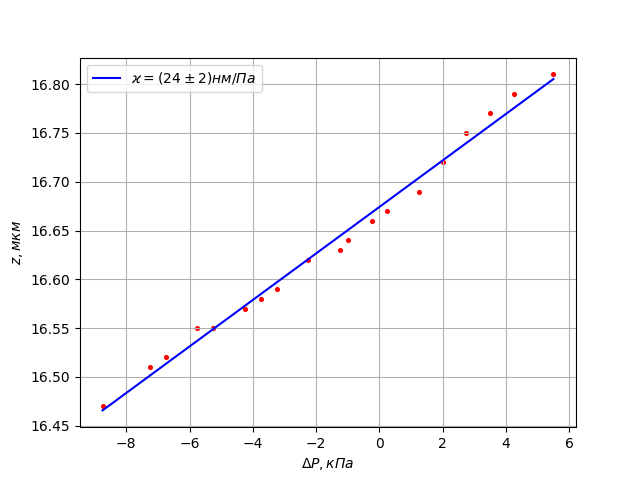
\includegraphics[scale=0.9]{z(P).png}}
			\caption{График зависимости $\triangle P$(z)}
		\end{figure}
		
		
		\item По следующей формуле перейдём от делений компенсатора к величине $\delta n$
		\begin{equation}
			\delta n = m\frac{\lambda}{l},
		\end{equation}
		при этом по рис. 2 имеем $ m = \frac{z}{k}$, где $k = 51 \pm 1$ мкм - тангенс угол наклона калибровочного графика, длина кюветы $l = 10 $см и длина волны, пропускаемая светофильтром $\lambda = 650 $нм. Тогда имеем
		
		\begin{equation}
			\delta n = \frac{z}{k} \frac{\lambda}{l} = 0,13 \cdot  z
		\end{equation}

		
		\item Определим среднюю поляризуемость молекулы воздуха:
		
		\begin{equation}
			\delta n = \frac{2 \pi \alpha}{kT} \triangle P
		\end{equation}
		
		\begin{equation}
			\alpha = \frac{\delta n kT}{2 \pi \triangle P} = \frac{0,13 \cdot z \cdot kT}{2 \pi \Delta P}=0,13 \cdot \varkappa \frac{ kT}{2 \pi} = 2,0 \cdot 10^{-30}, \hspace{1cm} \text{где T = 295} \pm {1^\circ}
		\end{equation}
		
		Табличное значение составляет $ \alpha = 1,7 \cdot 10^{-30}$
		
		\item Определим погрешность $ \alpha$.
		
		\begin{equation}
			\sigma_{\alpha} = \alpha\sqrt{ (\frac{\sigma_{\varkappa}}{\varkappa})^2 + (\frac{\sigma_{T}}{T})^2 } = 2 \hspace{1cm} \varepsilon = 10\%
		\end{equation}
		
		\item Определим показатель преломления воздуха Для $T = 293$ K и $P = 100$ кПа по формуле:
		\begin{equation}
			n = 1 + 2\pi\alpha \frac{P}{kT} = 1,00031
		\end{equation}
		
		Аналогично п. 5, погрешность определения показателя преломления составляет 
		\begin{equation}
			\sigma_n = 0,00003 
		\end{equation}
	
	\item Во вторую кювету запустим углекислый газ. Сразу после этого набежит разность хода, которая компенсируется поднятием компенсатора. Проведем серию экспериментов по заполнению камеры углекислым газом и определим набежавшую разность хода.
	
	\begin{longtable}{|c|c|c|c|c|c|c|}
		\hline
		№ & 1 & 2 & 3 & 4 & 5 & 6 \\ \hline
		$\Delta $, мм & 0,19 & 0,19 & 0,18 & 0,19 & 0,19 & 0,19 \\ \hline
		\caption{Полученные значения для разности хода при наличии в камере углекислого газа}
	\end{longtable}

	$$ \overline{\Delta} =  (0,19 \pm 0,02) \text{мм}$$ 	
	
	Так как $n_2 - n_1 = \delta n$, а $\delta n = \frac{\overline{\Delta}}{l}$ 
	
	Тогда 
	\begin{equation}
		n_{CO2} = n +  \frac{\overline{\Delta}}{l}= 1,00031 + 0,00016 = 1,00047 \pm 0,00005
	\end{equation} 
		
	\end{enumerate}
	
	\textbf{Обсуждение результатов и выводы: }\\
	
	В ходе данной работы мы познакомились с интерферометром Жамена, изучили его устройство. С помощью данного интерферометра смогли рассчитать поляризуемость $\alpha = (2,0 \pm 0,2) \cdot 10^{-30}$ и как следствие показатель преломления воздуха $n = (1,00031 \pm 0,00003)$. Полученные результаты сходятся в пределах погрешности с табличными  $\alpha_0 = 1,7 \cdot 10^{-30}$, n = 1,00029. Также по добавочной разности хода мы смогли определить показатель преломления углекислого газа $n_{CO2} = 1,00047 \pm 0,00005$, которое совпадает в пределах погрешности с табличным значением $n_{CO2} = 1,00045$.
	
	
	
	
	
	
	
	
	
	
	
	
	
	
	
	
	
	
	
	
	
	\end{document}